\subsection{Hyperblock}

通过RK算法,可以将无环的控制流图中的所有分支全部删除,并且转换为谓词执行。控制流图中的环对应于程序中的循环,几乎每一个程序都有循环,我们有的时候还是希望能对有环的控制流图进行处理。对于给定的控制流图,我们并不总是想要将整个流图中的所有分支删除,而是选择性的删除一部分分支。

要选择性地进行if-conversion,就是根据需要对控制流图中的基本块进行挑选,可以在控制流图中圈出一部分基本块,通过RK算法对这一部分基本块之间的分支进行消除,而保留其他部分的分支。可以把不经常被执行的基本块,或者太过长的基本块排除在外,而把经常执行又短小精悍的基本块包含在内,这样就能提高性能。如何选择基本块是策略问题,在本章不做详细讨论。

由于分支消除需要执行RK算法,所以对基本块的选择必须满足RK算法能够正确被执行的必要条件:只有一个入口。满足条件的基本块的集合称为Hyperblock。
\begin{definition}[Hyperblock]
Hyperblock是一个谓词化的基本块的集合,这个集合只有一个入口,但是可以有多个出口。
\end{definition}

虽然Hyperblock对基本块的选择提出了严格的限制,但是仍然可以通过一些变换将不满足Hyperblock定义的的基本块的集合转化为Hyperblock,这样就给基本块的选取提供了较大的自由度。

将对Hyperblock定义的违背分为两种情况:(1) 从外部跳入,(2) 内部存在循环。对于第一种情况的处理方法是\textbf{尾复制(tail duplication)},对于第二种情况的处理方法是\textbf{循环剥离(loop peeling)}。

尾复制从每一个由外部跳到内部的分支(跳转到这些块的入口处的分支排除)出发,沿着控制流图,将这些分支的所有直接或间接后继标记出来,然后将所有标记的基本块复制到外部,并将跳转到内部的分支重定向为跳转到其外部副本。如\fref{fig:taildup}所示,图中(a)是分支选择的结果,(b)是尾复制以后的结果,(c)是if-conversion之后的结果。
\begin{figure}
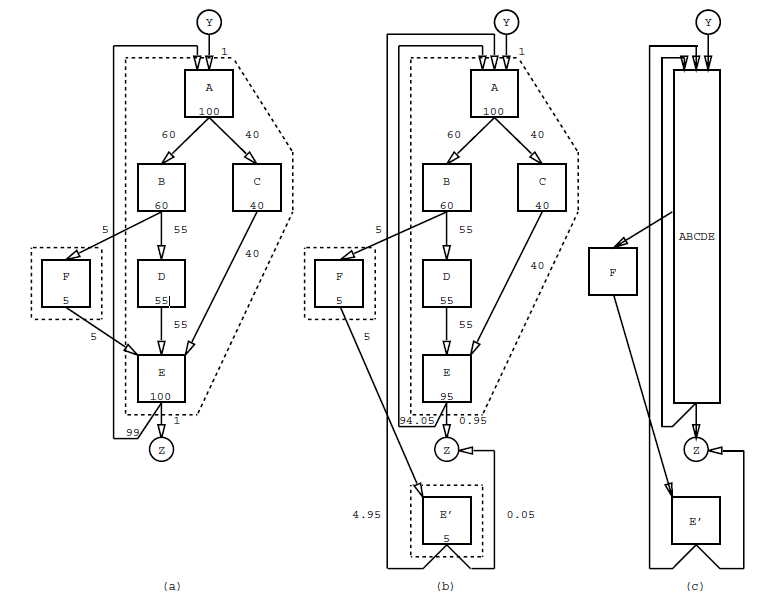
\includegraphics[width=\linewidth]{mechanism/hyperblock-td}
\caption{\label{fig:taildup} 尾复制}
\end{figure}

循环剥离则是将循环体以及其后继复制一份到外部,并将造成循环的跳转重定向到外部,这样循环的头一轮迭代留在内部被谓词化,而其后的几轮迭代则被移到外部执行。如\fref{fig:looppeeling}所示,图中(a)是分支选择的结果,(b)是循环剥离以后的结果。
\begin{figure}
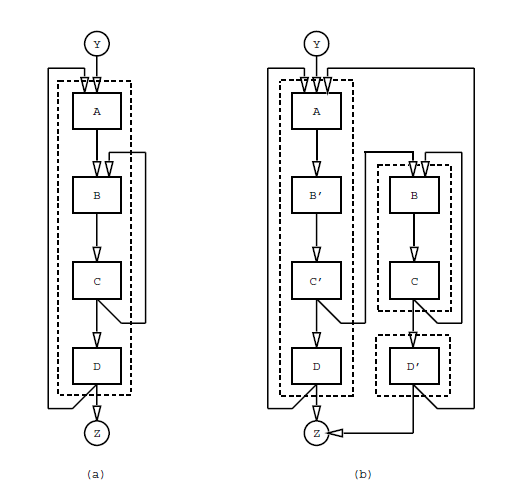
\includegraphics[width=\linewidth]{mechanism/hyperblock-lp}
\caption{\label{fig:looppeeling} 循环剥离}
\end{figure}
